\begin{frame}{Neural Network -- Functionality}

% \maketag{un/SUPERVISED} 
\maketag{regression | classification}
\maketag{non/parametric}
\maketag{BLACK-BOX} \maketag{feature selection}

\medskip

\highlight{General idea}
\begin{itemize}
  \item A \textbf{neural network (NN)} is a model architecture loosely inspired by 
  the human brain. It consists of various \textbf{neurons}, organized in 
  \textbf{layers} assembled through weighted functional connections. 
  \item Batches of data enter in the \textbf{input layer} and sequentially pass 
  through $h$ \textbf{hidden layers}, each of which performs a linear 
  \textbf{transformation} $\phi^{(j)}$and a non-linear \textbf{activation} 
  $\sigma^{(j)}$, thus creating intermediary representations of the data.
  \item The \textbf{output layer} yields predictions after a final transformation $\phi $ and 
  scaling $\tau$.
  \item The resulting loss is used to update the weights for the next 
  \textbf{epoch}.
\end{itemize}

\medskip
 
\highlight{Hypothesis space} ~~
$$\Hspace = \left\{ \fx: \fx = \tau \circ \phi \circ \sigma^{(h)} \circ
\phi^{(h)} \circ \sigma^{(h - 1)} \circ \phi^{(h - 1)} \circ ... \circ 
\sigma^{(1)} \circ \phi^{(1)} (\xv) \right\}$$

\smallskip

\begin{minipage}{0.25\textwidth}
  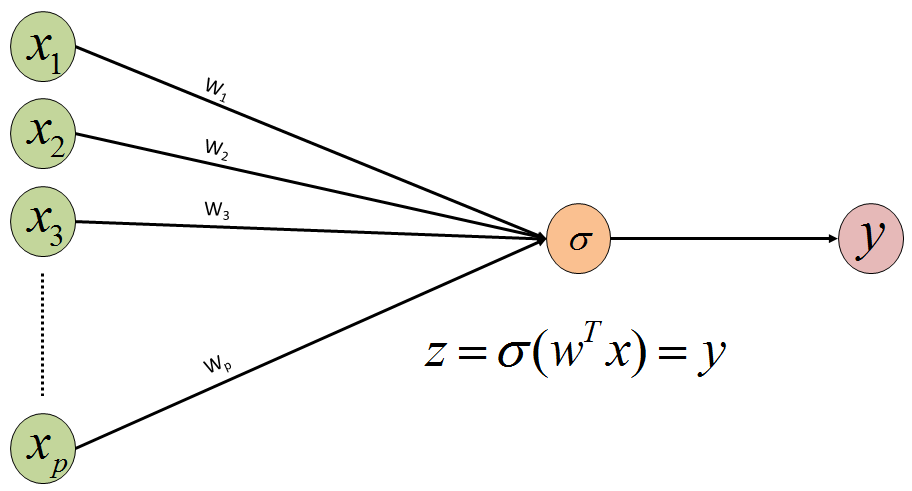
\includegraphics[width=0.9\textwidth]{figure/nn-single-neuron}
\end{minipage}%
\begin{minipage}{0.25\textwidth}
  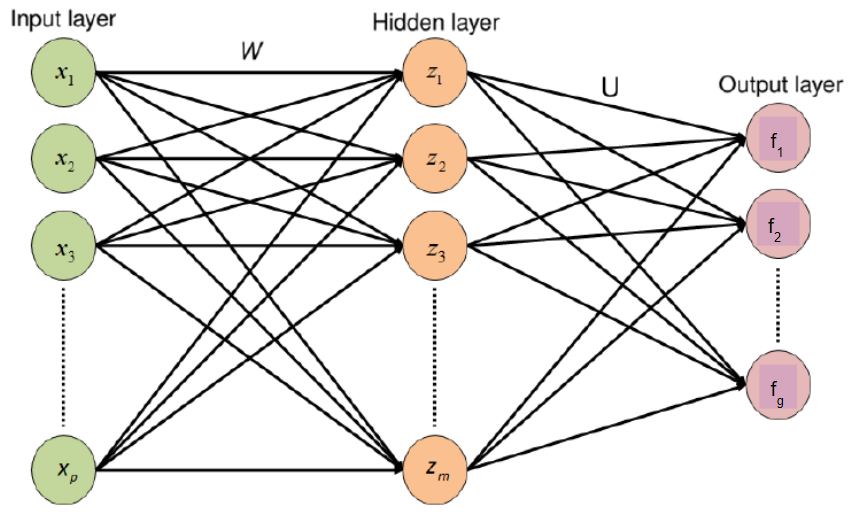
\includegraphics[width=0.9\textwidth]{figure/nn-feedforward}
\end{minipage}%
\begin{minipage}{0.5\textwidth}
  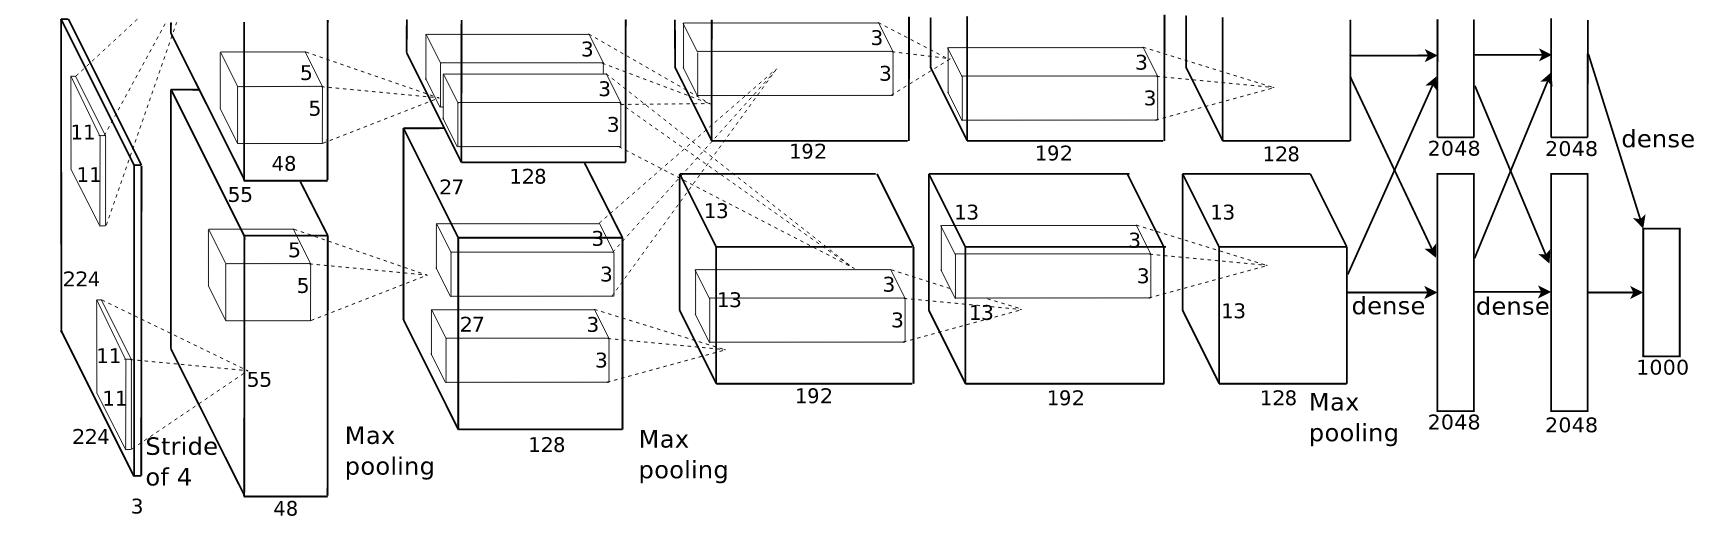
\includegraphics[width=\textwidth]{figure/nn-cnn-1}
\end{minipage}

\tiny
\textit{Left}: a single neuron, \textit{middle}: feedforward network with one 
hidden layer, \textit{right}: convolutional network

\end{frame}

% ------------------------------------------------------------------------------

\begin{frame}{Neural Network -- Functionality}

\footnotesize

\highlight{Empirical risk} ~~
\textcolor{blue}{Any \textbf{differentiable} loss function}

\medskip

\highlight{Optimization}

NNs are optimized by \textbf{backpropagation} which consists of two steps:
\begin{itemize}
  \item \textbf{Forward pass}: Predict result with current weights and 
  compute empirical risk according to chosen loss function. 
  \item \textbf{Backward pass}: Calculate error contribution of each weight by 
  means of gradient descent -- which essentially means applying the chain rule
  to the composition of functions applied in each layer -- and update weights 
  accordingly. 
\end{itemize}

\medskip

\highlight{Hyperparameters}

\begin{itemize}
  \item Number of hidden \textbf{layers} (depth), number of \textbf{neurons} 
  per layer
  \item \textbf{Activation} function(s)
  \item \textbf{Learning rate} for backpropagation
  \item Number of iterations (\textbf{epochs}), \textbf{batch} size
  \item Initial \textbf{weights} 
  \item ...
\end{itemize}

\medskip

% \highlight{Runtime behavior} ~~ \textcolor{blue}{???}

\end{frame}

% ------------------------------------------------------------------------------

\begin{frame}{Neural Network -- Pro's \& Con's}

\footnotesize

\begin{columns}[onlytextwidth]
  \begin{column}{0.5\textwidth}
    \highlight{Advantages}
    \footnotesize
    \begin{itemize}
      \positem Able to solve \textbf{complex, non-linear} regression or 
      classification problems
      \positem Therefore, typically very good \textbf{performance}
      \positem Built-in \textbf{feature extraction} - obtained by intermediary
      representations
      \positem Suitable for \textbf{unstructured} data (e. g. image, audio, 
      text data)
      \positem Easy handling of \textbf{high-dimensional} or \textbf{missing} 
      data
      \positem \textbf{Parallelizable} structure
    \end{itemize}
  \end{column}

  \begin{column}{0.5\textwidth}
    \highlight{Disadvantages}
    \footnotesize
    \begin{itemize}
      \negitem Computationally \textbf {expensive} \\
      $\rightarrow$ slow to train and forecast
      \negitem Large \textbf{amounts} of data required 
      \negitem \textbf{Faster-than-linear} scaling of weight matrices with 
      increased network size 
      \negitem Network architecture requiring much \textbf{expertise} in tuning
      \negitem \textbf{Black-box} model -- hard to interpret or explain
      \negitem Tendency towards \textbf{overfitting}
      
    \end{itemize}
  \end{column}
\end{columns}

\vfill

\small

\conclbox{Able to learn extremely complex functions, but computationally 
expensive and hard to get right}

\end{frame}

% ------------------------------------------------------------------------------

\begin{frame}{Neural Network -- Practical hints}

\footnotesize

\highlight{Types of neural networks (RNNs, CNNs)}

\begin{itemize}
  \item \textbf{Recurrent neural networks (RNNs}: Deep NN that make use of 
  \textbf{sequential} information with temporal \textbf{dependencies} \\
  $\rightarrow$ Frequently applied to \textbf{natural language processing}
  \item \textbf{Convolutional neural networks (CNNs)}: Regularized version of the 
  fully connected feed-forward NN (where each neuron is connected to all 
  neurons of the subsequent layer) that abstracts inputs to feature maps via 
  \textbf{convolution} \\
  $\rightarrow$ Frequently applied to \textbf{image recognition}

\end{itemize}

\medskip

\highlight{Problem of neural architecture search (NAS)}

NN are \textbf{not off-the-shelf} methods -- the network architecture needs to 
be tailored to each problem anew \\
$\rightarrow$ Automated machine learning attempts to learn architectures

\medskip
 
\highlight{Implementation}

\begin{itemize}
  \item \textbf{R:} package \texttt{neuralnet}
  \item \textbf{Python:} libraries \texttt{PyTorch}, \texttt{keras}
\end{itemize}

\end{frame}